% Options for packages loaded elsewhere
% Options for packages loaded elsewhere
\PassOptionsToPackage{unicode}{hyperref}
\PassOptionsToPackage{hyphens}{url}
%
\documentclass[
  11pt,
  ignorenonframetext,
  aspectratio=169,
]{beamer}
\newif\ifbibliography
\usepackage{pgfpages}
\setbeamertemplate{caption}[numbered]
\setbeamertemplate{caption label separator}{: }
\setbeamercolor{caption name}{fg=normal text.fg}
\beamertemplatenavigationsymbolsempty
% remove section numbering
\setbeamertemplate{part page}{
  \centering
  \begin{beamercolorbox}[sep=16pt,center]{part title}
    \usebeamerfont{part title}\insertpart\par
  \end{beamercolorbox}
}
\setbeamertemplate{section page}{
  \centering
  \begin{beamercolorbox}[sep=12pt,center]{section title}
    \usebeamerfont{section title}\insertsection\par
  \end{beamercolorbox}
}
\setbeamertemplate{subsection page}{
  \centering
  \begin{beamercolorbox}[sep=8pt,center]{subsection title}
    \usebeamerfont{subsection title}\insertsubsection\par
  \end{beamercolorbox}
}
% Prevent slide breaks in the middle of a paragraph
\widowpenalties 1 10000
\raggedbottom
\AtBeginPart{
  \frame{\partpage}
}
\AtBeginSection{
  \ifbibliography
  \else
    \frame{\sectionpage}
  \fi
}
\AtBeginSubsection{
  \frame{\subsectionpage}
}
\usepackage{iftex}
\ifPDFTeX
  \usepackage[T1]{fontenc}
  \usepackage[utf8]{inputenc}
  \usepackage{textcomp} % provide euro and other symbols
\else % if luatex or xetex
  \usepackage{unicode-math} % this also loads fontspec
  \defaultfontfeatures{Scale=MatchLowercase}
  \defaultfontfeatures[\rmfamily]{Ligatures=TeX,Scale=1}
\fi
\usepackage{lmodern}

\ifPDFTeX\else
  % xetex/luatex font selection
\fi
% Use upquote if available, for straight quotes in verbatim environments
\IfFileExists{upquote.sty}{\usepackage{upquote}}{}
\IfFileExists{microtype.sty}{% use microtype if available
  \usepackage[]{microtype}
  \UseMicrotypeSet[protrusion]{basicmath} % disable protrusion for tt fonts
}{}
\makeatletter
\@ifundefined{KOMAClassName}{% if non-KOMA class
  \IfFileExists{parskip.sty}{%
    \usepackage{parskip}
  }{% else
    \setlength{\parindent}{0pt}
    \setlength{\parskip}{6pt plus 2pt minus 1pt}}
}{% if KOMA class
  \KOMAoptions{parskip=half}}
\makeatother

\usepackage{color}
\usepackage{fancyvrb}
\newcommand{\VerbBar}{|}
\newcommand{\VERB}{\Verb[commandchars=\\\{\}]}
\DefineVerbatimEnvironment{Highlighting}{Verbatim}{commandchars=\\\{\}}
% Add ',fontsize=\small' for more characters per line
\usepackage{framed}
\definecolor{shadecolor}{RGB}{241,243,245}
\newenvironment{Shaded}{\begin{snugshade}}{\end{snugshade}}
\newcommand{\AlertTok}[1]{\textcolor[rgb]{0.68,0.00,0.00}{#1}}
\newcommand{\AnnotationTok}[1]{\textcolor[rgb]{0.37,0.37,0.37}{#1}}
\newcommand{\AttributeTok}[1]{\textcolor[rgb]{0.40,0.45,0.13}{#1}}
\newcommand{\BaseNTok}[1]{\textcolor[rgb]{0.68,0.00,0.00}{#1}}
\newcommand{\BuiltInTok}[1]{\textcolor[rgb]{0.00,0.23,0.31}{#1}}
\newcommand{\CharTok}[1]{\textcolor[rgb]{0.13,0.47,0.30}{#1}}
\newcommand{\CommentTok}[1]{\textcolor[rgb]{0.37,0.37,0.37}{#1}}
\newcommand{\CommentVarTok}[1]{\textcolor[rgb]{0.37,0.37,0.37}{\textit{#1}}}
\newcommand{\ConstantTok}[1]{\textcolor[rgb]{0.56,0.35,0.01}{#1}}
\newcommand{\ControlFlowTok}[1]{\textcolor[rgb]{0.00,0.23,0.31}{\textbf{#1}}}
\newcommand{\DataTypeTok}[1]{\textcolor[rgb]{0.68,0.00,0.00}{#1}}
\newcommand{\DecValTok}[1]{\textcolor[rgb]{0.68,0.00,0.00}{#1}}
\newcommand{\DocumentationTok}[1]{\textcolor[rgb]{0.37,0.37,0.37}{\textit{#1}}}
\newcommand{\ErrorTok}[1]{\textcolor[rgb]{0.68,0.00,0.00}{#1}}
\newcommand{\ExtensionTok}[1]{\textcolor[rgb]{0.00,0.23,0.31}{#1}}
\newcommand{\FloatTok}[1]{\textcolor[rgb]{0.68,0.00,0.00}{#1}}
\newcommand{\FunctionTok}[1]{\textcolor[rgb]{0.28,0.35,0.67}{#1}}
\newcommand{\ImportTok}[1]{\textcolor[rgb]{0.00,0.46,0.62}{#1}}
\newcommand{\InformationTok}[1]{\textcolor[rgb]{0.37,0.37,0.37}{#1}}
\newcommand{\KeywordTok}[1]{\textcolor[rgb]{0.00,0.23,0.31}{\textbf{#1}}}
\newcommand{\NormalTok}[1]{\textcolor[rgb]{0.00,0.23,0.31}{#1}}
\newcommand{\OperatorTok}[1]{\textcolor[rgb]{0.37,0.37,0.37}{#1}}
\newcommand{\OtherTok}[1]{\textcolor[rgb]{0.00,0.23,0.31}{#1}}
\newcommand{\PreprocessorTok}[1]{\textcolor[rgb]{0.68,0.00,0.00}{#1}}
\newcommand{\RegionMarkerTok}[1]{\textcolor[rgb]{0.00,0.23,0.31}{#1}}
\newcommand{\SpecialCharTok}[1]{\textcolor[rgb]{0.37,0.37,0.37}{#1}}
\newcommand{\SpecialStringTok}[1]{\textcolor[rgb]{0.13,0.47,0.30}{#1}}
\newcommand{\StringTok}[1]{\textcolor[rgb]{0.13,0.47,0.30}{#1}}
\newcommand{\VariableTok}[1]{\textcolor[rgb]{0.07,0.07,0.07}{#1}}
\newcommand{\VerbatimStringTok}[1]{\textcolor[rgb]{0.13,0.47,0.30}{#1}}
\newcommand{\WarningTok}[1]{\textcolor[rgb]{0.37,0.37,0.37}{\textit{#1}}}

\usepackage{longtable,booktabs,array}
\newcounter{none} % for unnumbered tables
\usepackage{calc} % for calculating minipage widths
\usepackage{caption}
% Make caption package work with longtable
\makeatletter
\def\fnum@table{\tablename~\thetable}
\makeatother
\usepackage{graphicx}
\makeatletter
\newsavebox\pandoc@box
\newcommand*\pandocbounded[1]{% scales image to fit in text height/width
  \sbox\pandoc@box{#1}%
  \Gscale@div\@tempa{\textheight}{\dimexpr\ht\pandoc@box+\dp\pandoc@box\relax}%
  \Gscale@div\@tempb{\linewidth}{\wd\pandoc@box}%
  \ifdim\@tempb\p@<\@tempa\p@\let\@tempa\@tempb\fi% select the smaller of both
  \ifdim\@tempa\p@<\p@\scalebox{\@tempa}{\usebox\pandoc@box}%
  \else\usebox{\pandoc@box}%
  \fi%
}
% Set default figure placement to htbp
\def\fps@figure{htbp}
\makeatother





\setlength{\emergencystretch}{3em} % prevent overfull lines

\providecommand{\tightlist}{%
  \setlength{\itemsep}{0pt}\setlength{\parskip}{0pt}}



 


\setbeamertemplate{navigation symbols}{}
\setbeamertemplate{footline}[frame number]
\setbeamertemplate{itemize items}[circle]
\setbeamertemplate{itemize subitem}[triangle]
\setbeamercolor{frametitle}{fg=black}
\setbeamerfont{frametitle}{series=\bfseries}
\newcommand{\indep}{\perp\!\!\!\perp}
\usepackage{booktabs}
\usepackage{tikz}
\usetikzlibrary{arrows.meta,positioning,calc}
\tikzset{
  dnode/.style={circle,draw,thick,minimum size=9mm,inner sep=1pt,font=\small},
  unode/.style={circle,draw,thick,dashed,minimum size=9mm,inner sep=1pt,font=\small},
  bnode/.style={rectangle,draw,thick,fill=gray!25,minimum size=9mm,inner sep=3pt,font=\small},
  de/.style={-{Stealth[length=2.2mm]},thick},
  dde/.style={-{Stealth[length=2.2mm]},thick,dashed}
}
% shrink code input (fancyvrb) and code output (verbatim)
\usepackage{fancyvrb}
\fvset{fontsize=\scriptsize}
\makeatletter
\def\verbatim@font{\scriptsize\ttfamily}
\makeatother
\makeatletter
\@ifpackageloaded{caption}{}{\usepackage{caption}}
\AtBeginDocument{%
\ifdefined\contentsname
  \renewcommand*\contentsname{Table of contents}
\else
  \newcommand\contentsname{Table of contents}
\fi
\ifdefined\listfigurename
  \renewcommand*\listfigurename{List of Figures}
\else
  \newcommand\listfigurename{List of Figures}
\fi
\ifdefined\listtablename
  \renewcommand*\listtablename{List of Tables}
\else
  \newcommand\listtablename{List of Tables}
\fi
\ifdefined\figurename
  \renewcommand*\figurename{Figure}
\else
  \newcommand\figurename{Figure}
\fi
\ifdefined\tablename
  \renewcommand*\tablename{Table}
\else
  \newcommand\tablename{Table}
\fi
}
\@ifpackageloaded{float}{}{\usepackage{float}}
\floatstyle{ruled}
\@ifundefined{c@chapter}{\newfloat{codelisting}{h}{lop}}{\newfloat{codelisting}{h}{lop}[chapter]}
\floatname{codelisting}{Listing}
\newcommand*\listoflistings{\listof{codelisting}{List of Listings}}
\makeatother
\makeatletter
\makeatother
\makeatletter
\@ifpackageloaded{caption}{}{\usepackage{caption}}
\@ifpackageloaded{subcaption}{}{\usepackage{subcaption}}
\makeatother

\usepackage{bookmark}
\IfFileExists{xurl.sty}{\usepackage{xurl}}{} % add URL line breaks if available
\urlstyle{same}
\hypersetup{
  pdftitle={Directed Acyclic Graphs},
  pdfauthor={Professor Ji-Woong Chung},
  hidelinks,
  pdfcreator={LaTeX via pandoc}}


\title{\texorpdfstring{Directed Acyclic
Graphs}{Directed Acyclic Graphs}}
\subtitle{\texorpdfstring{BUSS975: Causal Inference in Financial
Research}{BUSS975: Causal Inference in Financial Research}}
\author{Professor Ji-Woong Chung}
\date{}
\institute{Korea University}

\begin{document}
\frame{\titlepage}


\begin{frame}[fragile]{Acknowledgments and readings}
\protect\phantomsection\label{acknowledgments-and-readings}
\begin{itemize}
\tightlist
\item
  These slides are based on Scott Cunningham, \emph{Causal Inference:
  The Remix} (2nd ed.), Chapter 3, ``Directed Acyclic Graphs.''

  \begin{itemize}
  \tightlist
  \item
    Free online: \texttt{https://mixtape.scunning.com}
  \end{itemize}
\item
  The backdoor criterion and the adjustment formula follow Pearl (2009).
\end{itemize}
\end{frame}

\begin{frame}{Outline}
\protect\phantomsection\label{outline}
\begin{enumerate}
\tightlist
\item
  Why graphs?
\item
  DAG notation
\item
  Three elemental structures
\item
  Backdoor paths and adjustment
\item
  Collider bias
\item
  Bad controls
\item
  Neutral controls and precision
\item
  What DAGs cannot do
\end{enumerate}
\end{frame}

\section{Why Graphs?}\label{why-graphs}

\begin{frame}{Where we left off}
\protect\phantomsection\label{where-we-left-off}
\begin{itemize}
\tightlist
\item
  Last lecture: a causal effect is a property of the data \textbf{plus
  the assignment mechanism}.
\item
  The potential outcomes framework gave us:

  \begin{itemize}
  \tightlist
  \item
    precise \textbf{estimands} --- \(ATE\), \(ATT\), \(ATU\);
  \item
    a decomposition of what goes wrong --- selection bias and
    heterogeneity bias;
  \item
    a gold standard --- randomization, which makes
    \((Y^1,Y^0) \indep D\).
  \end{itemize}
\item
  What it did \textbf{not} give us: a systematic way to answer the
  single most common question in empirical work.
\end{itemize}

\begin{center}
\emph{``What should I control for?''}
\end{center}
\end{frame}

\begin{frame}{The question every referee asks}
\protect\phantomsection\label{the-question-every-referee-asks}
\begin{itemize}
\tightlist
\item
  A typical referee report: \emph{``The authors should control for firm
  size, leverage, industry, and profitability.''}
\item
  Is that good advice? The honest answer in most papers is:
  \textbf{nobody knows}.
\item
  Common (bad) heuristics:

  \begin{itemize}
  \tightlist
  \item
    ``Control for everything you have.'' --- Wrong, and this lecture
    shows why.
  \item
    ``Control for anything correlated with both \(D\) and \(Y\).'' ---
    Closer, but still wrong.
  \item
    ``More controls make the estimate more credible.'' --- Emphatically
    wrong.
  \end{itemize}
\item
  Adding a control can \textbf{remove} bias, \textbf{add} bias, or
  \textbf{flip the sign} of your estimate.
\item
  To tell which, you need a language for your assumptions about the
  data-generating process.
\end{itemize}
\end{frame}

\begin{frame}{What a DAG is for}
\protect\phantomsection\label{what-a-dag-is-for}
\begin{itemize}
\tightlist
\item
  A \textbf{directed acyclic graph} is a picture of your causal
  assumptions.
\item
  Once drawn, it delivers --- mechanically, by rules you can check ---

  \begin{itemize}
  \tightlist
  \item
    which variables you \textbf{must} control for,
  \item
    which variables you \textbf{must not} control for,
  \item
    whether your causal effect is identified \textbf{at all} from
    observational data.
  \end{itemize}
\item
  The DAG does not tell you whether your assumptions are \emph{true}.
  Nothing does.
\item
  What it does is make them \textbf{explicit, communicable, and
  refutable} --- so a referee can disagree with your \emph{assumptions}
  rather than your \emph{taste in controls}.
\end{itemize}
\end{frame}

\begin{frame}{This lecture \ldots{}}
\protect\phantomsection\label{this-lecture}
By the end you will be able to explain, precisely, why the following is
true:

\vspace{0.5em}

\begin{center}
\emph{You can run a perfectly randomized experiment, add one perfectly measured\\
control variable, and get an estimate with the wrong sign.}
\end{center}

\vspace{0.5em}

\begin{itemize}
\tightlist
\item
  We will simulate exactly this in §6, ``Bad Controls.''
\item
  If controlling for things can do that, ``control for everything'' is
  not a strategy --- it is a coin flip.
\end{itemize}
\end{frame}

\section{DAG Notation}\label{dag-notation}

\begin{frame}{Nodes and arrows}
\protect\phantomsection\label{nodes-and-arrows}
\begin{itemize}
\tightlist
\item
  A DAG has \textbf{nodes} (random variables) and \textbf{directed
  edges} (arrows).
\item
  An arrow \(X \to Y\) means: \(X\) exerts a \textbf{direct causal
  effect} on \(Y\) --- direct meaning \emph{not} routed through any
  other variable in the graph.
\end{itemize}

\begin{center}
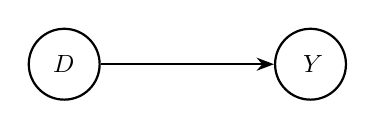
\begin{tikzpicture}[node distance=22mm]
\node[dnode] (D) {$D$};
\node[dnode, right=of D] (Y) {$Y$};
\draw[de] (D) -- (Y);
\end{tikzpicture}
\end{center}

\begin{itemize}
\tightlist
\item
  Read: relationship lending (\(D\)) affects firm investment (\(Y\)).
\item
  The graph is \textbf{non-parametric}: it says nothing about magnitude,
  sign, linearity, or functional form. Only \emph{whether} an effect
  exists.
\end{itemize}
\end{frame}

\begin{frame}{The missing arrow is the assumption}
\protect\phantomsection\label{the-missing-arrow-is-the-assumption}
\begin{itemize}
\tightlist
\item
  Drawing an arrow is a weak claim: ``\(X\) may affect \(Y\).''
\item
  \textbf{Omitting} an arrow is a strong claim: ``\(X\) has \emph{no}
  effect on \(Y\), for any unit, of any size.''
\item
  This is the opposite of how we usually read a regression table, and it
  is the most important thing to remember about DAGs.
\item
  So the interesting content of a DAG is in the arrows you \textbf{did
  not draw}.
\item
  Corollary: a DAG with arrows everywhere is honest but useless ---
  nothing is identified. Progress requires exclusions, and exclusions
  require \textbf{institutional knowledge}.
\end{itemize}
\end{frame}

\begin{frame}{Acyclicity}
\protect\phantomsection\label{acyclicity}
\begin{itemize}
\tightlist
\item
  ``Acyclic'' = no directed path leads from a variable back to itself.
\item
  Forbidden:
\end{itemize}

\begin{center}
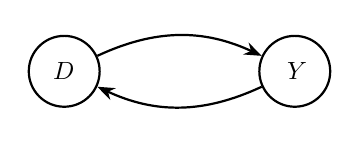
\begin{tikzpicture}[node distance=20mm]
\node[dnode] (D) {$D$};
\node[dnode, right=of D] (Y) {$Y$};
\draw[de] (D) to[bend left=25] (Y);
\draw[de] (Y) to[bend left=25] (D);
\end{tikzpicture}
\end{center}

\begin{itemize}
\tightlist
\item
  This is a real restriction for finance, where equilibrium feedback is
  everywhere: leverage and performance, price and demand, coverage and
  returns.
\item
  The usual fix is \textbf{time}:
  \(\text{Leverage}_t \to \text{Perf}_{t+1} \to \text{Leverage}_{t+2}\)
  is acyclic.
\item
  Genuine simultaneity is beyond what a DAG can express. We return to
  this in §8.
\end{itemize}
\end{frame}

\begin{frame}{Observed and unobserved variables}
\protect\phantomsection\label{observed-and-unobserved-variables}
\begin{itemize}
\tightlist
\item
  Solid circle = \textbf{observed}; dashed circle = \textbf{unobserved}.
\end{itemize}

\begin{center}
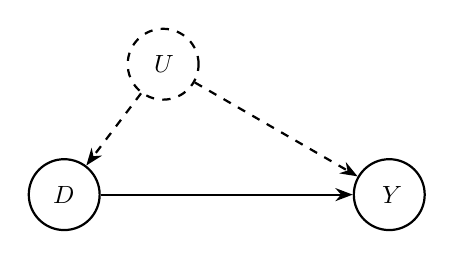
\begin{tikzpicture}[node distance=18mm]
\node[dnode] (D) {$D$};
\node[dnode, right=32mm of D] (Y) {$Y$};
\node[unode, above right=10mm and 6mm of D] (U) {$U$};
\draw[de] (D) -- (Y);
\draw[dde] (U) -- (D);
\draw[dde] (U) -- (Y);
\end{tikzpicture}
\end{center}

\begin{itemize}
\tightlist
\item
  \(U\) might be managerial talent, firm culture, private information,
  or local demand.
\item
  The distinction matters enormously: a variable you cannot measure
  cannot be conditioned on, so it cannot be used to block anything.
\item
  Much of this course is about what to do when a \(U\) like this exists.
\end{itemize}
\end{frame}

\begin{frame}{Paths}
\protect\phantomsection\label{paths}
\begin{itemize}
\tightlist
\item
  A \textbf{path} is any sequence of edges connecting two nodes,
  \emph{ignoring the direction of the arrows}.
\item
  A \textbf{directed (causal) path} follows the arrows from start to
  finish.
\end{itemize}

\begin{center}
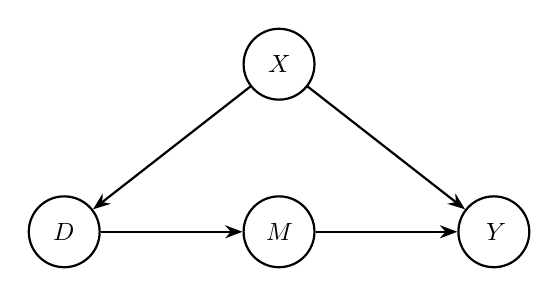
\begin{tikzpicture}[node distance=18mm]
\node[dnode] (D) {$D$};
\node[dnode, right=of D] (M) {$M$};
\node[dnode, right=of M] (Y) {$Y$};
\node[dnode, above=12mm of M] (X) {$X$};
\draw[de] (D) -- (M);
\draw[de] (M) -- (Y);
\draw[de] (X) -- (D);
\draw[de] (X) -- (Y);
\end{tikzpicture}
\end{center}

\begin{itemize}
\tightlist
\item
  \(D \to M \to Y\) is a directed path (this is the causal effect).
\item
  \(D \leftarrow X \to Y\) is a path but \textbf{not} a directed path
  --- yet it still generates correlation between \(D\) and \(Y\).
\item
  \textbf{Association flows along paths regardless of arrow direction.
  Causation flows only along directed paths.}
\end{itemize}
\end{frame}

\begin{frame}{Where DAGs come from}
\protect\phantomsection\label{where-dags-come-from}
\begin{itemize}
\tightlist
\item
  A DAG is \textbf{not} derived from the data. The data cannot tell you
  which way the arrows point.
\item
  It comes from: economic theory, institutional detail, prior empirical
  work, and knowledge of how \emph{your specific dataset} was assembled.
\item
  Two researchers with different institutional knowledge will draw
  different DAGs and reach different conclusions --- and that is the
  point. The disagreement is now \textbf{visible and arguable}.
\item
  Practical advice: draw the DAG \emph{before} you run the regression.
  If you cannot draw it, you do not yet understand your identification
  strategy.
\end{itemize}
\end{frame}

\begin{frame}{Controlling for is not setting}
\protect\phantomsection\label{controlling-for-is-not-setting}
\begin{itemize}
\tightlist
\item
  A recurring confusion, worth naming before we build the machinery.
\item
  \textbf{Controlling for \(X\)} filters the data: ``among firms that
  \emph{happen} to have \(X = x\).'' The population changes --- we keep
  a subpopulation, which may be special in ways we cannot see.
\item
  \textbf{Setting \(X\)} intervenes: ``if we \emph{assigned} \(X = x\)
  to every firm.'' The population stays fixed; only \(X\) moves.
\item
  Prediction needs only the first. Causal inference needs the second.
\item
  In graph terms, setting \(X\) means \textbf{deleting every arrow into
  \(X\)} --- \(X\) is no longer caused by its parents; it is caused by
  us.

  \begin{itemize}
  \tightlist
  \item
    That is exactly what a randomized experiment does physically: the
    coin, not the firm's characteristics, becomes the parent of \(D\).
  \item
    It is why randomization needs no controls. There are no arrows left
    to block.
  \end{itemize}
\end{itemize}
\end{frame}

\begin{frame}{Ratings predict default; ratings do not prevent it}
\protect\phantomsection\label{ratings-predict-default-ratings-do-not-prevent-it}
\begin{itemize}
\tightlist
\item
  Let \(Y = 1\) if a firm defaults within five years, and let \(X\) be
  its credit rating.
\item
  \textbf{Filtering}: among AAA issuers, default is rare. Ratings are
  superb \emph{predictors} --- selling this number is a profitable
  business.
\item
  \textbf{Setting}: suppose a regulator relabelled every junk issuer
  AAA. Default rates would barely move. The label is not the cash flows.
\item
  Filtering \textbf{selects} firms that were already creditworthy;
  setting \textbf{changes the label} and leaves creditworthiness
  untouched.
\item
  The causal effect is not exactly zero --- ratings do move borrowing
  costs, covenant triggers, and forced buying and selling by investors
  whose mandates are rating-based --- but nothing like the AAA-to-junk
  gap.

  \begin{itemize}
  \tightlist
  \item
    (Kisgen and Strahan 2010: when the SEC certified DBRS in 2003,
    yields moved \textbf{39bp per notch} --- the label alone, with
    fundamentals unchanged.)
  \end{itemize}
\item
  Ask of any empirical result: \emph{is this a filter, or an
  intervention?}
\end{itemize}
\end{frame}

\section{Three Elemental Structures}\label{three-elemental-structures}

\begin{frame}{Every DAG is built from three pieces}
\protect\phantomsection\label{every-dag-is-built-from-three-pieces}
Any path, however long, is a chain of three-node segments of exactly
three types.

\begin{center}
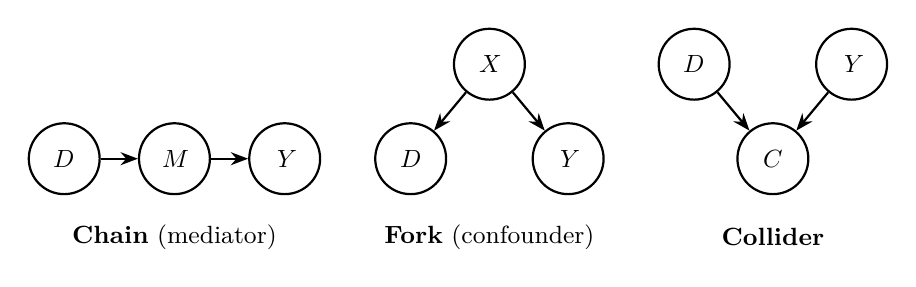
\begin{tikzpicture}
% chain
\node[dnode] (D1) at (0,0) {$D$};
\node[dnode] (M1) at (1.4,0) {$M$};
\node[dnode] (Y1) at (2.8,0) {$Y$};
\draw[de] (D1) -- (M1);
\draw[de] (M1) -- (Y1);
\node[font=\small] at (1.4,-1.0) {\textbf{Chain} (mediator)};
% fork
\node[dnode] (D2) at (4.4,0) {$D$};
\node[dnode] (Y2) at (6.4,0) {$Y$};
\node[dnode] (X2) at (5.4,1.2) {$X$};
\draw[de] (X2) -- (D2);
\draw[de] (X2) -- (Y2);
\node[font=\small] at (5.4,-1.0) {\textbf{Fork} (confounder)};
% collider
\node[dnode] (D3) at (8.0,1.2) {$D$};
\node[dnode] (Y3) at (10.0,1.2) {$Y$};
\node[dnode] (C3) at (9.0,0) {$C$};
\draw[de] (D3) -- (C3);
\draw[de] (Y3) -- (C3);
\node[font=\small] at (9.0,-1.0) {\textbf{Collider}};
\end{tikzpicture}
\end{center}

\begin{itemize}
\tightlist
\item
  A \textbf{collider} on a path is a node where two arrowheads meet:
  \(\to C \leftarrow\).
\item
  Whether a node is a collider is a property of the \textbf{path}, not
  of the variable.
\end{itemize}
\end{frame}

\begin{frame}{Chain: \(D \to M \to Y\)}
\protect\phantomsection\label{chain-d-to-m-to-y}
\begin{itemize}
\tightlist
\item
  \(M\) is a \textbf{mediator}: the causal effect of \(D\) travels
  \emph{through} it.
\item
  The path is \textbf{open} by default --- \(D\) and \(Y\) are
  correlated, and the correlation is causal.
\item
  Conditioning on \(M\) \textbf{closes} the path --- and thereby
  destroys the very effect you are trying to measure.
\item
  Finance example: a credit shock raises investment, which raises
  employment.

  \begin{itemize}
  \tightlist
  \item
    \(\text{Credit} \to \text{Investment} \to \text{Employment}\).
  \item
    Controlling for investment when estimating the effect of credit on
    employment removes most of the answer.
  \end{itemize}
\item
  \textbf{Do not control for mediators} when you want the total effect.
\end{itemize}
\end{frame}

\begin{frame}{Fork: \(D \leftarrow X \to Y\)}
\protect\phantomsection\label{fork-d-leftarrow-x-to-y}
\begin{itemize}
\tightlist
\item
  \(X\) is a \textbf{confounder}: a common cause of both treatment and
  outcome.
\item
  The path is \textbf{open} by default --- \(D\) and \(Y\) are
  correlated, but the correlation is \textbf{not} causal.
\item
  Conditioning on \(X\) \textbf{closes} the path and removes the bias.
\item
  This is exactly omitted variable bias from last lecture, drawn as a
  picture.
\item
  Finance example: firm quality drives both whether a firm has a lending
  relationship and how much it invests.
\item
  \textbf{Do control for confounders} --- if you can measure them.
\end{itemize}
\end{frame}

\begin{frame}{Collider: \(D \to C \leftarrow Y\)}
\protect\phantomsection\label{collider-d-to-c-leftarrow-y}
\begin{itemize}
\tightlist
\item
  \(C\) is a \textbf{collider}: a common \emph{effect} of treatment and
  outcome.
\item
  The path is \textbf{closed} by default --- \(D\) and \(Y\) are
  \emph{not} correlated through it.
\item
  Conditioning on \(C\) \textbf{opens} the path and \emph{creates} a
  correlation that did not exist.
\item
  This is the one with no counterpart in your regression training, and
  it is where most damage is done.
\item
  Finance example: skill and luck are independent, but both determine
  whether a fund survives. Study only survivors and skill and luck
  become correlated.
\item
  \textbf{Do not control for colliders} --- and note that ``control
  for'' includes \emph{sample selection}.
\end{itemize}
\end{frame}

\begin{frame}{The one table to memorize}
\protect\phantomsection\label{the-one-table-to-memorize}
\begin{center}
\small
\begin{tabular}{lcccc}
\toprule
& & \textbf{Association} & \textbf{Conditioning} & \textbf{Should} \\
Structure & Shape & \textbf{flows already?} & \textbf{on middle node} & \textbf{you?} \\
\midrule
Chain (mediator)  & $D \to M \to Y$        & Yes, \emph{causal}   & \textbf{blocks} it & \textbf{No} \\
Fork (confounder) & $D \leftarrow X \to Y$ & Yes, \emph{spurious} & \textbf{blocks} it & \textbf{Yes} \\
Collider          & $D \to C \leftarrow Y$ & No                   & \textbf{opens} it  & \textbf{No} \\
\bottomrule
\end{tabular}
\end{center}

\vspace{0.4em}

\begin{itemize}
\tightlist
\item
  Column 3 asks whether \(D\) and \(Y\) are \emph{already} correlated
  through this structure; column 4, what conditioning does to that.
\item
  Only the \textbf{fork} is worth conditioning on: it is the only
  structure where association flows and is \emph{not} the effect you
  want.
\item
  Mediators and colliders are both ``leave alone'' --- for opposite
  reasons. Blocking a mediator deletes the answer; opening a collider
  invents one.
\item
  Conditioning on a \textbf{descendant} of a collider partially opens it
  too. A proxy for a collider is still a collider.
\end{itemize}
\end{frame}

\section{Backdoor Paths and the Backdoor
Criterion}\label{backdoor-paths-and-the-backdoor-criterion}

\begin{frame}{Backdoor paths}
\protect\phantomsection\label{backdoor-paths}
\begin{itemize}
\tightlist
\item
  A \textbf{backdoor path} is a path connecting \(D\) and \(Y\) that
  begins with an arrow pointing \emph{into} \(D\).
\item
  Compare: \(D \to Y\) leaves \(D\) through an arrow pointing
  \emph{out}, so it is a front-door --- the causal path.
\item
  Backdoor paths generate correlation without causation --- ``back
  doors'' through which association leaks.
\item
  Identification strategy in one sentence:
\end{itemize}

\begin{center}
\emph{Leave every directed path from $D$ to $Y$ open.\\
Close every backdoor path.}
\end{center}

\begin{itemize}
\tightlist
\item
  The \textbf{backdoor criterion}: a set of variables \(\mathbf{Z}\)
  identifies the causal effect of \(D\) on \(Y\) if

  \begin{enumerate}
  \tightlist
  \item
    \(\mathbf{Z}\) blocks every backdoor path from \(D\) to \(Y\), and
  \item
    \(\mathbf{Z}\) contains no descendant of \(D\).
  \end{enumerate}
\item
  Condition 2 is what rules out mediators and post-treatment colliders.
\end{itemize}
\end{frame}

\begin{frame}{A DAG: Example}
\protect\phantomsection\label{a-dag-example}
Effect of a bank \textbf{relationship} (\(D\)) on firm
\textbf{investment} (\(Y\)).

\begin{center}
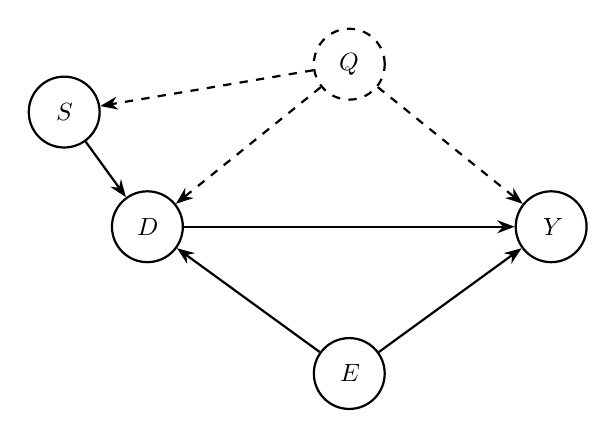
\begin{tikzpicture}[node distance=16mm]
\node[dnode] (D) {$D$};
\node[dnode, right=42mm of D] (Y) {$Y$};
\node[unode, above=16mm of $(D)!0.5!(Y)$] (Q) {$Q$};
\node[dnode, above left=8mm and 4mm of D] (S) {$S$};
\node[dnode, below=14mm of $(D)!0.5!(Y)$] (E) {$E$};
\draw[de] (D) -- (Y);
\draw[dde] (Q) -- (D);
\draw[dde] (Q) -- (Y);
\draw[de] (S) -- (D);
\draw[dde] (Q) -- (S);
\draw[de] (E) -- (D);
\draw[de] (E) -- (Y);
\end{tikzpicture}
\end{center}

\vspace{-0.3em}

\begin{itemize}
\tightlist
\item
  \(Q\) = firm quality (\textbf{unobserved}), \(S\) = firm size, \(E\) =
  local economic conditions.
\end{itemize}
\end{frame}

\begin{frame}{Enumerate the paths}
\protect\phantomsection\label{enumerate-the-paths}
From the previous DAG:

\begin{enumerate}
\tightlist
\item
  \(D \to Y\) --- \textbf{directed}. Leave open; this is the estimand.
\item
  \(D \leftarrow Q \to Y\) --- backdoor, open (fork at \(Q\)).
\item
  \(D \leftarrow S \leftarrow Q \to Y\) --- backdoor, open (chain then
  fork).
\item
  \(D \leftarrow E \to Y\) --- backdoor, open (fork at \(E\)).
\end{enumerate}

\vspace{0.5em}

\begin{itemize}
\tightlist
\item
  Conditioning on \(\{Q, E\}\) blocks paths 2, 3, and 4. Identified.
\item
  But \(Q\) is \textbf{unobserved}. So the achievable set is
  \(\{S, E\}\):

  \begin{itemize}
  \tightlist
  \item
    blocks path 3 (at \(S\)) and path 4 (at \(E\)),
  \item
    leaves path 2 \textbf{open}.
  \end{itemize}
\item
  Conclusion: the effect is \textbf{not identified} by controlling for
  observables.
\item
  That conclusion --- reached before running anything --- is the DAG
  earning its keep.
\end{itemize}
\end{frame}

\begin{frame}[fragile]{Simulation: the fork, and closing it}
\protect\phantomsection\label{simulation-the-fork-and-closing-it}
\(Q \to D\), \(Q \to Y\), \(D \to Y\) with a true effect of \(2\).

\begin{Shaded}
\begin{Highlighting}[]
\FunctionTok{set.seed}\NormalTok{(}\DecValTok{975}\NormalTok{)}
\NormalTok{n    }\OtherTok{\textless{}{-}} \DecValTok{100000}
\NormalTok{qual }\OtherTok{\textless{}{-}} \FunctionTok{rnorm}\NormalTok{(n)                    }\CommentTok{\# firm quality (the confounder)}
\NormalTok{D    }\OtherTok{\textless{}{-}} \FloatTok{0.6} \SpecialCharTok{*}\NormalTok{ qual }\SpecialCharTok{+} \FunctionTok{rnorm}\NormalTok{(n)       }\CommentTok{\# relationship lending}
\NormalTok{Y    }\OtherTok{\textless{}{-}} \DecValTok{2} \SpecialCharTok{*}\NormalTok{ D }\SpecialCharTok{+} \FloatTok{1.5} \SpecialCharTok{*}\NormalTok{ qual }\SpecialCharTok{+} \FunctionTok{rnorm}\NormalTok{(n)   }\CommentTok{\# TRUE effect of D on Y is 2}

\NormalTok{b }\OtherTok{\textless{}{-}} \ControlFlowTok{function}\NormalTok{(f) }\FunctionTok{unname}\NormalTok{(}\FunctionTok{coef}\NormalTok{(}\FunctionTok{lm}\NormalTok{(f))[}\DecValTok{2}\NormalTok{])}
\FunctionTok{round}\NormalTok{(}\FunctionTok{c}\NormalTok{(}\AttributeTok{naive =} \FunctionTok{b}\NormalTok{(Y }\SpecialCharTok{\textasciitilde{}}\NormalTok{ D), }\AttributeTok{control\_Q =} \FunctionTok{b}\NormalTok{(Y }\SpecialCharTok{\textasciitilde{}}\NormalTok{ D }\SpecialCharTok{+}\NormalTok{ qual)), }\DecValTok{3}\NormalTok{)}
\end{Highlighting}
\end{Shaded}

\begin{verbatim}
    naive control_Q 
    2.662     2.001 
\end{verbatim}

\begin{itemize}
\tightlist
\item
  Leaving the backdoor open: the estimate is too large by about
  \(0.66\).
\item
  Blocking it at \(Q\): we recover the truth. This is OVB from last
  lecture, now read off a graph.
\item
  Here ``blocking'' just means putting \(Q\) in the regression. There is
  a more general way to do it --- reweighting rather than regressing ---
  which we take up with \textbf{inverse probability weighting} in the
  DiD lecture.
\end{itemize}
\end{frame}

\begin{frame}{Multiple valid strategies}
\protect\phantomsection\label{multiple-valid-strategies}
\begin{itemize}
\tightlist
\item
  Often several different sets satisfy the backdoor criterion.
\item
  Any of them gives an \textbf{unbiased} estimate --- so choose among
  them on \textbf{precision}.
\item
  Rule of thumb: prefer the set that includes strong predictors of
  \(Y\).

  \begin{itemize}
  \tightlist
  \item
    They do not change identification; they shrink residual variance and
    tighten standard errors.
  \end{itemize}
\item
  This is the legitimate version of ``add controls to make the estimate
  sharper'' --- legitimate precisely because you verified the backdoor
  criterion \emph{first}.
\item
  The illegitimate version, adding controls and hoping, is what the rest
  of this lecture is about.
\end{itemize}
\end{frame}

\section{Collider Bias}\label{collider-bias}

\begin{frame}{Colliders create correlation out of nothing}
\protect\phantomsection\label{colliders-create-correlation-out-of-nothing}
\begin{itemize}
\tightlist
\item
  The claim that surprises people: conditioning on a collider makes
  \textbf{independent} variables dependent.
\item
  Intuition. Suppose a fund survives only if
  \(\text{skill} + \text{luck}\) is high enough.

  \begin{itemize}
  \tightlist
  \item
    Among survivors, a manager with low skill \emph{must} have had high
    luck --- otherwise they would not be in the sample.
  \item
    So within survivors, skill and luck are \textbf{negatively}
    correlated, though they are independent in the population.
  \end{itemize}
\item
  Nothing was manipulated, no arrow was drawn. The correlation is
  manufactured entirely by \textbf{who is in the sample}.
\end{itemize}
\end{frame}

\begin{frame}{Survivorship as a collider}
\protect\phantomsection\label{survivorship-as-a-collider}
\begin{center}
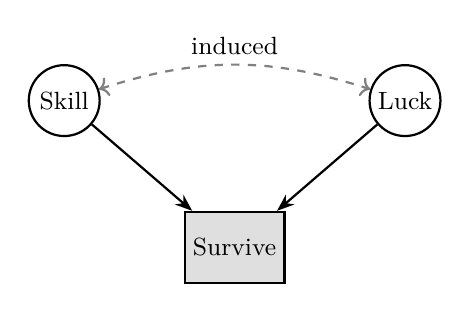
\begin{tikzpicture}[node distance=18mm]
\node[dnode] (S) {Skill};
\node[dnode, right=34mm of S] (L) {Luck};
\node[bnode, below=14mm of $(S)!0.5!(L)$] (V) {Survive};
\draw[de] (S) -- (V);
\draw[de] (L) -- (V);
\draw[dde, <->, gray] (S) to[bend left=18] node[above,font=\small,black]{induced} (L);
\end{tikzpicture}
\end{center}

\begin{itemize}
\tightlist
\item
  Grey box = we conditioned on it (here, by studying only surviving
  funds).
\item
  Skill \(\to\) Survive \(\leftarrow\) Luck is a collider. It was
  closed. We opened it.
\end{itemize}
\end{frame}

\begin{frame}[fragile]{Simulation: the surviving-fund fallacy}
\protect\phantomsection\label{simulation-the-surviving-fund-fallacy}
\begin{Shaded}
\begin{Highlighting}[]
\FunctionTok{set.seed}\NormalTok{(}\DecValTok{975}\NormalTok{)}
\NormalTok{n     }\OtherTok{\textless{}{-}} \DecValTok{100000}
\NormalTok{skill }\OtherTok{\textless{}{-}} \FunctionTok{rnorm}\NormalTok{(n)                       }\CommentTok{\# independent...}
\NormalTok{luck  }\OtherTok{\textless{}{-}} \FunctionTok{rnorm}\NormalTok{(n)                       }\CommentTok{\# ...by construction}
\NormalTok{perf  }\OtherTok{\textless{}{-}}\NormalTok{ skill }\SpecialCharTok{+}\NormalTok{ luck}
\NormalTok{surv  }\OtherTok{\textless{}{-}}\NormalTok{ perf }\SpecialCharTok{\textgreater{}} \FunctionTok{quantile}\NormalTok{(perf, }\FloatTok{0.80}\NormalTok{)    }\CommentTok{\# only the top 20\% survive}

\FunctionTok{round}\NormalTok{(}\FunctionTok{c}\NormalTok{(}\AttributeTok{cor\_all       =} \FunctionTok{cor}\NormalTok{(skill, luck),}
        \AttributeTok{cor\_survivors =} \FunctionTok{cor}\NormalTok{(skill[surv], luck[surv])), }\DecValTok{3}\NormalTok{)}
\end{Highlighting}
\end{Shaded}

\begin{verbatim}
      cor_all cor_survivors 
       -0.003        -0.640 
\end{verbatim}

\vspace{-0.5em}

\begin{Shaded}
\begin{Highlighting}[]
\FunctionTok{round}\NormalTok{(}\FunctionTok{c}\NormalTok{(}\AttributeTok{slope\_all       =} \FunctionTok{unname}\NormalTok{(}\FunctionTok{coef}\NormalTok{(}\FunctionTok{lm}\NormalTok{(perf }\SpecialCharTok{\textasciitilde{}}\NormalTok{ skill))[}\DecValTok{2}\NormalTok{]),}
        \AttributeTok{slope\_survivors =} \FunctionTok{unname}\NormalTok{(}\FunctionTok{coef}\NormalTok{(}\FunctionTok{lm}\NormalTok{(perf[surv] }\SpecialCharTok{\textasciitilde{}}\NormalTok{ skill[surv]))[}\DecValTok{2}\NormalTok{])), }\DecValTok{3}\NormalTok{)}
\end{Highlighting}
\end{Shaded}

\begin{verbatim}
      slope_all slope_survivors 
          0.997           0.358 
\end{verbatim}

\begin{itemize}
\tightlist
\item
  Skill and luck: independent in the population, correlated \(-0.64\)
  among survivors.
\item
  The return to skill looks like \(0.36\) instead of \(1.00\) ---
  understated by nearly two thirds.
\end{itemize}
\end{frame}

\begin{frame}{This is not a hypothetical}
\protect\phantomsection\label{this-is-not-a-hypothetical}
\begin{itemize}
\tightlist
\item
  The same structure appears throughout empirical finance, usually
  unnoticed:

  \begin{itemize}
  \tightlist
  \item
    \textbf{Fund performance studies} on surviving funds.
  \item
    \textbf{Compustat / Execucomp}: a firm appears only if it listed and
    survived. Listing is caused by size, quality, and opportunity --- a
    collider.
  \item
    \textbf{M\&A studies} conditioned on \textbf{completed} deals:
    completion is caused by bidder synergies \emph{and} target
    resistance.
  \item
    \textbf{Rated firms only}: a firm is rated when it chooses to issue
    public debt.
  \item
    \textbf{IPO samples}: going public is a common effect of quality and
    market conditions.
  \end{itemize}
\item
  Empirical finance treats these as a list of separate warnings ---
  survivorship bias, sample coverage, deal completion. They are
  \textbf{one structural error}: conditioning on a collider.
\item
  The DAG turns a folklore checklist into a rule you can check.
\end{itemize}
\end{frame}

\begin{frame}{Selection \emph{is} conditioning}
\protect\phantomsection\label{selection-is-conditioning}
\begin{itemize}
\tightlist
\item
  Emphasize: you do not need to type a variable into a regression to
  condition on it.
\item
  You condition on a variable whenever you

  \begin{itemize}
  \tightlist
  \item
    include it as a control,
  \item
    stratify or match on it,
  \item
    \textbf{drop observations} based on it,
  \item
    or use a dataset that was \textbf{assembled} using it.
  \end{itemize}
\item
  The last one is the dangerous case, because it is invisible in your
  code.
\end{itemize}

\vspace{0.3em}

\textbf{Example.} Your sample is the CRSP--Compustat merged file. A firm
appears only if it (i) listed on a US exchange and (ii) filed accounts
that got matched. Both are consequences of size, age, and quality ---
the same things driving your outcome. You conditioned on a collider
without writing a single line of code that mentions it.

\vspace{0.3em}

\begin{itemize}
\tightlist
\item
  Practical advice: write \emph{how the sample was constructed} into the
  DAG, as nodes. Sample-construction filters are conditioning
  statements.
\end{itemize}
\end{frame}

\begin{frame}{Sign reversal: the classic example}
\protect\phantomsection\label{sign-reversal-the-classic-example}
\begin{itemize}
\tightlist
\item
  Cunningham's example, following Pearl: does gender discrimination
  lower wages?
\item
  Discrimination pushes women into lower-paying occupations, \emph{and}
  lowers pay directly. Ability raises both occupation and wage.
\end{itemize}

\begin{center}
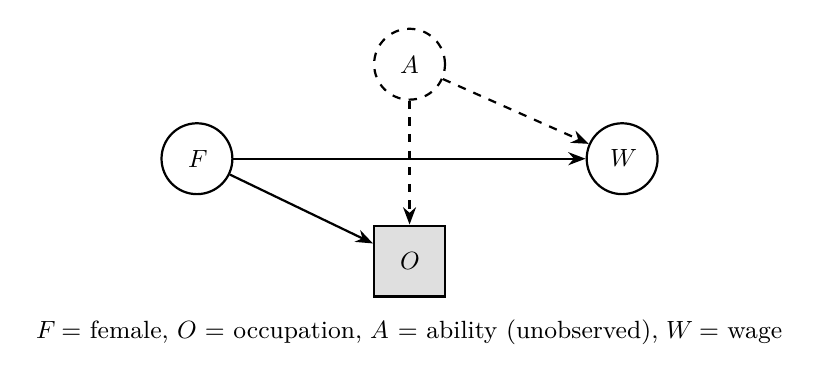
\begin{tikzpicture}
\node[dnode] (F) at (0,0) {$F$};
\node[dnode] (W) at (5.4,0) {$W$};
\node[bnode] (O) at (2.7,-1.3) {$O$};
\node[unode] (A) at (2.7,1.2) {$A$};
\draw[de] (F) -- (W);
\draw[de] (F) -- (O);
\draw[dde] (A) -- (O);
\draw[dde] (A) -- (W);
\node[font=\small] at (2.7,-2.2) {$F$ = female, $O$ = occupation, $A$ = ability (unobserved), $W$ = wage};
\end{tikzpicture}
\end{center}

\begin{itemize}
\tightlist
\item
  \(O\) is a \textbf{collider} on \(F \to O \leftarrow A \to W\). It is
  also a \textbf{mediator} on \(F \to O \to W\).
\item
  Controlling for it does both bad things at once: blocks part of the
  real effect, and opens a spurious path.
\end{itemize}
\end{frame}

\begin{frame}[fragile]{Simulating the sign reversal}
\protect\phantomsection\label{simulating-the-sign-reversal}
\begin{Shaded}
\begin{Highlighting}[]
\FunctionTok{set.seed}\NormalTok{(}\DecValTok{975}\NormalTok{)}
\NormalTok{n       }\OtherTok{\textless{}{-}} \DecValTok{10000}
\NormalTok{female  }\OtherTok{\textless{}{-}} \FunctionTok{rbinom}\NormalTok{(n, }\DecValTok{1}\NormalTok{, }\FloatTok{0.5}\NormalTok{)}
\NormalTok{ability }\OtherTok{\textless{}{-}} \FunctionTok{rnorm}\NormalTok{(n)                                    }\CommentTok{\# unobserved in practice}
\NormalTok{occ     }\OtherTok{\textless{}{-}} \DecValTok{1} \SpecialCharTok{+} \DecValTok{2}\SpecialCharTok{*}\NormalTok{ability }\SpecialCharTok{{-}} \DecValTok{2}\SpecialCharTok{*}\NormalTok{female  }\SpecialCharTok{+} \FunctionTok{rnorm}\NormalTok{(n)        }\CommentTok{\# discrimination {-}\textgreater{} worse occupation}
\NormalTok{wage    }\OtherTok{\textless{}{-}} \DecValTok{1} \SpecialCharTok{{-}} \DecValTok{1}\SpecialCharTok{*}\NormalTok{female }\SpecialCharTok{+} \DecValTok{1}\SpecialCharTok{*}\NormalTok{occ }\SpecialCharTok{+} \DecValTok{2}\SpecialCharTok{*}\NormalTok{ability }\SpecialCharTok{+} \FunctionTok{rnorm}\NormalTok{(n) }\CommentTok{\# direct effect of discrimination = {-}1}

\NormalTok{b }\OtherTok{\textless{}{-}} \ControlFlowTok{function}\NormalTok{(f) }\FunctionTok{unname}\NormalTok{(}\FunctionTok{coef}\NormalTok{(}\FunctionTok{lm}\NormalTok{(f))[}\DecValTok{2}\NormalTok{])}
\FunctionTok{round}\NormalTok{(}\FunctionTok{c}\NormalTok{(}\AttributeTok{none        =} \FunctionTok{b}\NormalTok{(wage }\SpecialCharTok{\textasciitilde{}}\NormalTok{ female),}
        \AttributeTok{occ\_only    =} \FunctionTok{b}\NormalTok{(wage }\SpecialCharTok{\textasciitilde{}}\NormalTok{ female }\SpecialCharTok{+}\NormalTok{ occ),}
        \AttributeTok{occ\_ability =} \FunctionTok{b}\NormalTok{(wage }\SpecialCharTok{\textasciitilde{}}\NormalTok{ female }\SpecialCharTok{+}\NormalTok{ occ }\SpecialCharTok{+}\NormalTok{ ability)), }\DecValTok{3}\NormalTok{)}
\end{Highlighting}
\end{Shaded}

\begin{verbatim}
       none    occ_only occ_ability 
     -2.983       0.591      -0.996 
\end{verbatim}

\begin{itemize}
\tightlist
\item
  True \textbf{direct} effect \(= -1\); true \textbf{total} effect
  \(= -1 + 1\times(-2) = -3\).
\end{itemize}
\end{frame}

\begin{frame}{Reading the sign reversal}
\protect\phantomsection\label{reading-the-sign-reversal}
\begin{itemize}
\tightlist
\item
  \textbf{No controls} \(\approx -3\): recovers the \emph{total} effect.
  Correct, if total is what you want.
\item
  \textbf{Control for occupation} \(\approx +0.6\): \textbf{the sign
  flips.} Within an occupation, a woman must have had higher ability to
  get there --- so the female dummy now partly proxies for ability,
  which raises wages.
\item
  \textbf{Control for occupation and ability} \(\approx -1\): recovers
  the direct effect, because conditioning on \(A\) closes the path that
  conditioning on \(O\) opened.
\item
  The rescue only worked because ability was \textbf{observable in the
  simulation}. In your data it is not.
\item
  The finance version is exactly this shape: study a shock's effect on
  firm value, control for leverage, and unobserved quality does the work
  that ability does here.
\end{itemize}
\end{frame}

\section{Bad Controls}\label{bad-controls}

\begin{frame}{The bad control problem}
\protect\phantomsection\label{the-bad-control-problem}
\begin{itemize}
\tightlist
\item
  A \textbf{bad control} is a variable that is itself affected by the
  treatment.
\item
  Last lecture we previewed this and deferred the explanation. Here it
  is:

  \begin{itemize}
  \tightlist
  \item
    if \(D \to X\), then \(X\) is a descendant of \(D\);
  \item
    conditioning on it violates part 2 of the backdoor criterion;
  \item
    it either blocks part of the causal effect (if \(X\) is a mediator)
    or opens a collider path (if \(X\) has another parent).
  \end{itemize}
\item
  The second case is the nasty one, because it can happen even when
  \(D\) was \textbf{randomly assigned}.
\end{itemize}
\end{frame}

\begin{frame}{Randomization does not protect you}
\protect\phantomsection\label{randomization-does-not-protect-you}
\begin{center}
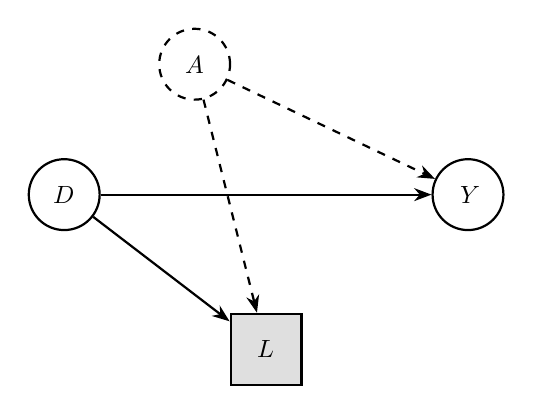
\begin{tikzpicture}[node distance=18mm]
\node[dnode] (D) {$D$};
\node[dnode, right=42mm of D] (Y) {$Y$};
\node[bnode, below=15mm of $(D)!0.5!(Y)$] (L) {$L$};
\node[unode, above right=10mm and 10mm of D] (A) {$A$};
\draw[de] (D) -- (Y);
\draw[de] (D) -- (L);
\draw[dde] (A) -- (L);
\draw[dde] (A) -- (Y);
\end{tikzpicture}
\end{center}

\begin{itemize}
\tightlist
\item
  \(D\) = credit supply shock (\textbf{randomly assigned}), \(Y\) =
  investment, \(L\) = leverage, \(A\) = firm quality (unobserved).
\item
  Nothing points into \(D\): there are \textbf{no backdoor paths}. The
  naive regression is already correct.
\item
  But \(L\) is a collider on \(D \to L \leftarrow A \to Y\). Control for
  leverage and you open it.
\end{itemize}
\end{frame}

\begin{frame}[fragile]{Simulation: how to ruin an experiment}
\protect\phantomsection\label{simulation-how-to-ruin-an-experiment}
\begin{Shaded}
\begin{Highlighting}[]
\FunctionTok{set.seed}\NormalTok{(}\DecValTok{975}\NormalTok{)}
\NormalTok{n }\OtherTok{\textless{}{-}} \DecValTok{100000}
\NormalTok{D }\OtherTok{\textless{}{-}} \FunctionTok{rnorm}\NormalTok{(n)                     }\CommentTok{\# credit shock {-}{-} RANDOMLY ASSIGNED}
\NormalTok{A }\OtherTok{\textless{}{-}} \FunctionTok{rnorm}\NormalTok{(n)                     }\CommentTok{\# firm quality {-}{-} unobserved}
\NormalTok{L }\OtherTok{\textless{}{-}}\NormalTok{ D }\SpecialCharTok{+}\NormalTok{ A }\SpecialCharTok{+} \FunctionTok{rnorm}\NormalTok{(n)             }\CommentTok{\# leverage {-}{-} affected by treatment}
\NormalTok{Y }\OtherTok{\textless{}{-}} \DecValTok{1} \SpecialCharTok{*}\NormalTok{ D }\SpecialCharTok{+} \DecValTok{3} \SpecialCharTok{*}\NormalTok{ A }\SpecialCharTok{+} \FunctionTok{rnorm}\NormalTok{(n)     }\CommentTok{\# TRUE effect of D on Y is +1}

\NormalTok{b }\OtherTok{\textless{}{-}} \ControlFlowTok{function}\NormalTok{(f) }\FunctionTok{unname}\NormalTok{(}\FunctionTok{coef}\NormalTok{(}\FunctionTok{lm}\NormalTok{(f))[}\DecValTok{2}\NormalTok{])}
\FunctionTok{round}\NormalTok{(}\FunctionTok{c}\NormalTok{(}\AttributeTok{no\_controls     =} \FunctionTok{b}\NormalTok{(Y }\SpecialCharTok{\textasciitilde{}}\NormalTok{ D),}
        \AttributeTok{control\_L       =} \FunctionTok{b}\NormalTok{(Y }\SpecialCharTok{\textasciitilde{}}\NormalTok{ D }\SpecialCharTok{+}\NormalTok{ L),}
        \AttributeTok{control\_L\_and\_A =} \FunctionTok{b}\NormalTok{(Y }\SpecialCharTok{\textasciitilde{}}\NormalTok{ D }\SpecialCharTok{+}\NormalTok{ L }\SpecialCharTok{+}\NormalTok{ A)), }\DecValTok{3}\NormalTok{)}
\end{Highlighting}
\end{Shaded}

\begin{verbatim}
    no_controls       control_L control_L_and_A 
          0.993          -0.493           1.008 
\end{verbatim}

\begin{itemize}
\tightlist
\item
  Treatment was randomized. The true effect is \(+1\). One control
  variable turns it into \(-0.5\).
\item
  Nothing here is mismeasured, nonlinear, or small-sample.
  \(n = 100{,}000\) and the bias is structural.
\end{itemize}
\end{frame}

\begin{frame}{Reading the damage}
\protect\phantomsection\label{reading-the-damage}
\begin{itemize}
\tightlist
\item
  Without controls: \(D\) is randomized, no backdoor exists, estimate
  \(\approx 1\). Correct.
\item
  Adding \(L\): opens \(D \to L \leftarrow A \to Y\), and the estimate
  drops to \(-0.5\).
\item
  Adding \(A\) as well: closes the newly opened path, restoring \(+1\)
  --- but \(A\) is unobserved in any real study.
\item
  The lesson is not ``leverage is a bad control.'' It is:
\end{itemize}

\begin{center}
\emph{Whether a variable is a good control is not a property of the variable.\\
It is a property of its position in the graph.}
\end{center}
\end{frame}

\begin{frame}{Bad controls in finance}
\protect\phantomsection\label{bad-controls-in-finance}
Common post-treatment controls, and what they do:

\begin{itemize}
\tightlist
\item
  \textbf{Leverage / firm size / Tobin's Q} in a study of a shock that
  plausibly moves them.
\item
  \textbf{Analyst coverage} when studying disclosure --- disclosure
  changes coverage.
\item
  \textbf{Deal completion} in M\&A --- completion is post-announcement.
\item
  \textbf{Survival to \(t+1\)} in any panel with attrition.
\item
  \textbf{Post-treatment industry classification} for firms that change
  industries after treatment.
\end{itemize}

\vspace{0.4em}

\begin{itemize}
\tightlist
\item
  The operational rule from last lecture, now justified:
  \textbf{controls must be determined before treatment}.
\item
  When in doubt, report the specification without the questionable
  control. If the estimate moves a lot, you have learned something ---
  and you must explain which specification the DAG supports.
\end{itemize}
\end{frame}

\section{Neutral Controls and
Precision}\label{neutral-controls-and-precision}

\begin{frame}{Not every control matters}
\protect\phantomsection\label{not-every-control-matters}
\begin{itemize}
\tightlist
\item
  Some variables are neither confounders nor colliders. Conditioning on
  them changes nothing about bias.
\item
  Two useful cases:

  \begin{itemize}
  \tightlist
  \item
    \(X \to Y\) only (a predictor of the outcome, unrelated to \(D\)):
    \textbf{harmless and helpful} --- it reduces residual variance and
    tightens standard errors.
  \item
    \(X \to D\) only (a predictor of treatment, unrelated to \(Y\)):
    \textbf{harmless but harmful in practice} --- it absorbs variation
    in \(D\) and \emph{inflates} standard errors.
  \end{itemize}
\item
  The second is the seed of the weak-instrument and ``overcontrolling''
  problems you will meet in the IV lecture.
\end{itemize}
\end{frame}

\begin{frame}{Precision: the setup}
\protect\phantomsection\label{precision-the-setup}
\begin{center}
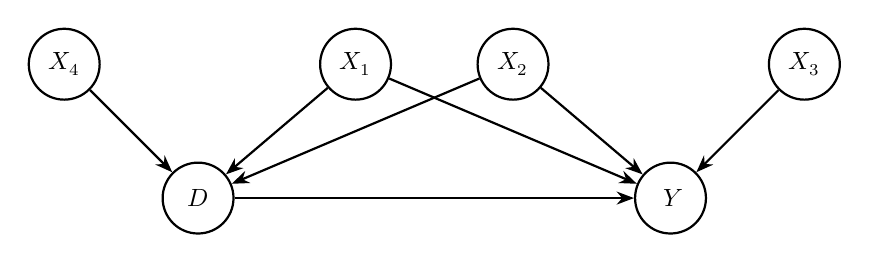
\begin{tikzpicture}
\node[dnode] (D)  at (0,0)     {$D$};
\node[dnode] (Y)  at (6,0)     {$Y$};
\node[dnode] (X1) at (2,1.7)   {$X_1$};
\node[dnode] (X2) at (4,1.7)   {$X_2$};
\node[dnode] (X4) at (-1.7,1.7) {$X_4$};
\node[dnode] (X3) at (7.7,1.7)  {$X_3$};
\draw[de] (D) -- (Y);
\draw[de] (X1) -- (D);
\draw[de] (X1) -- (Y);
\draw[de] (X2) -- (D);
\draw[de] (X2) -- (Y);
\draw[de] (X4) -- (D);
\draw[de] (X3) -- (Y);
\end{tikzpicture}
\end{center}

\begin{itemize}
\tightlist
\item
  \(X_1, X_2\) are \textbf{confounders} --- they point at both \(D\) and
  \(Y\). Any valid set must include them.
\item
  \(X_3\) points at \(Y\) only. \(X_4\) points at \(D\) only. Neither
  sits on a backdoor path, so \textbf{neither is needed} for
  identification.
\item
  All three sets below therefore satisfy the backdoor criterion. They
  differ only in precision.
\end{itemize}
\end{frame}

\begin{frame}[fragile]{Precision: simulating three valid strategies}
\protect\phantomsection\label{precision-simulating-three-valid-strategies}
\begin{Shaded}
\begin{Highlighting}[]
\FunctionTok{set.seed}\NormalTok{(}\DecValTok{975}\NormalTok{)}
\NormalTok{sim }\OtherTok{\textless{}{-}} \ControlFlowTok{function}\NormalTok{() \{}
\NormalTok{  n  }\OtherTok{\textless{}{-}} \DecValTok{1000}
\NormalTok{  x1 }\OtherTok{\textless{}{-}} \FunctionTok{rnorm}\NormalTok{(n); x2 }\OtherTok{\textless{}{-}} \FunctionTok{rnorm}\NormalTok{(n)                 }\CommentTok{\# confounders: {-}\textgreater{} D and {-}\textgreater{} Y}
\NormalTok{  x3 }\OtherTok{\textless{}{-}} \FunctionTok{rnorm}\NormalTok{(n)                                 }\CommentTok{\# predicts Y only}
\NormalTok{  x4 }\OtherTok{\textless{}{-}} \FunctionTok{rnorm}\NormalTok{(n)                                 }\CommentTok{\# predicts D only}
\NormalTok{  D  }\OtherTok{\textless{}{-}} \FloatTok{0.5}\SpecialCharTok{*}\NormalTok{x1 }\SpecialCharTok{+} \FloatTok{0.5}\SpecialCharTok{*}\NormalTok{x2 }\SpecialCharTok{+} \FloatTok{1.5}\SpecialCharTok{*}\NormalTok{x4 }\SpecialCharTok{+} \FunctionTok{rnorm}\NormalTok{(n)}
\NormalTok{  Y  }\OtherTok{\textless{}{-}} \DecValTok{2}\SpecialCharTok{*}\NormalTok{D }\SpecialCharTok{+} \DecValTok{2}\SpecialCharTok{*}\NormalTok{x1 }\SpecialCharTok{+} \DecValTok{2}\SpecialCharTok{*}\NormalTok{x2 }\SpecialCharTok{+} \DecValTok{4}\SpecialCharTok{*}\NormalTok{x3 }\SpecialCharTok{+} \FunctionTok{rnorm}\NormalTok{(n)      }\CommentTok{\# TRUE effect = 2}
\NormalTok{  b  }\OtherTok{\textless{}{-}} \ControlFlowTok{function}\NormalTok{(f) }\FunctionTok{unname}\NormalTok{(}\FunctionTok{coef}\NormalTok{(}\FunctionTok{lm}\NormalTok{(f))[}\DecValTok{2}\NormalTok{])}
  \FunctionTok{c}\NormalTok{(}\AttributeTok{minimal =} \FunctionTok{b}\NormalTok{(Y }\SpecialCharTok{\textasciitilde{}}\NormalTok{ D }\SpecialCharTok{+}\NormalTok{ x1 }\SpecialCharTok{+}\NormalTok{ x2),}
    \AttributeTok{plus\_x3 =} \FunctionTok{b}\NormalTok{(Y }\SpecialCharTok{\textasciitilde{}}\NormalTok{ D }\SpecialCharTok{+}\NormalTok{ x1 }\SpecialCharTok{+}\NormalTok{ x2 }\SpecialCharTok{+}\NormalTok{ x3),}
    \AttributeTok{plus\_x4 =} \FunctionTok{b}\NormalTok{(Y }\SpecialCharTok{\textasciitilde{}}\NormalTok{ D }\SpecialCharTok{+}\NormalTok{ x1 }\SpecialCharTok{+}\NormalTok{ x2 }\SpecialCharTok{+}\NormalTok{ x4))}
\NormalTok{\}}
\NormalTok{r }\OtherTok{\textless{}{-}} \FunctionTok{replicate}\NormalTok{(}\DecValTok{1000}\NormalTok{, }\FunctionTok{sim}\NormalTok{())}
\FunctionTok{round}\NormalTok{(}\FunctionTok{rbind}\NormalTok{(}\AttributeTok{mean =} \FunctionTok{apply}\NormalTok{(r, }\DecValTok{1}\NormalTok{, mean), }\AttributeTok{sd =} \FunctionTok{apply}\NormalTok{(r, }\DecValTok{1}\NormalTok{, sd)), }\DecValTok{4}\NormalTok{)}
\end{Highlighting}
\end{Shaded}

\begin{verbatim}
     minimal plus_x3 plus_x4
mean  1.9999  2.0002  1.9962
sd    0.0735  0.0172  0.1299
\end{verbatim}
\end{frame}

\begin{frame}{Reading the precision results}
\protect\phantomsection\label{reading-the-precision-results}
\begin{itemize}
\tightlist
\item
  All three are \textbf{unbiased} --- every mean is \(2.000\).
  Identification is settled; only variance differs.
\item
  Adding \(X_3\), which predicts \textbf{only \(Y\)}, cuts the standard
  deviation from \(0.074\) to \(0.017\) --- four times sharper. It soaks
  up residual variance without touching identification.
\item
  Adding \(X_4\), which predicts \textbf{only \(D\)}, raises it to
  \(0.130\) --- nearly twice as noisy. It absorbs the variation in \(D\)
  you were relying on.
\item
  Same bias, a sevenfold spread in precision.
\item
  \textbf{Practical guidance}:

  \begin{enumerate}
  \tightlist
  \item
    First use the DAG to find sets that identify the effect. That is
    about \emph{bias}.
  \item
    Then, among those sets, prefer strong predictors of \(Y\) and avoid
    strong predictors of \(D\) alone. That is about \emph{variance}.
  \end{enumerate}
\item
  Never reverse the order. Choosing controls by what tightens the
  standard error is how sign flips get published.
\item
  The \(X_4\) case is the seed of the weak-instrument problem in the IV
  lecture: an instrument is a variable that predicts \(D\) and nothing
  else.
\end{itemize}
\end{frame}

\section{What DAGs Cannot Do}\label{what-dags-cannot-do}

\begin{frame}{Honest limitations}
\protect\phantomsection\label{honest-limitations}
\begin{enumerate}
\tightlist
\item
  \textbf{DAGs do not test assumptions.} A DAG is an argument, not
  evidence. The data cannot tell you which way an arrow points.
\item
  \textbf{DAGs are non-parametric.} They tell you \emph{whether} an
  effect is identified, never how large it is, nor the functional form,
  nor the estimator.
\item
  \textbf{DAGs are acyclic.} Genuine simultaneity --- the equilibrium
  feedback that pervades finance --- cannot be drawn. Time-indexing
  helps; it does not always suffice.
\item
  \textbf{DAGs say nothing about magnitude.} A technically open backdoor
  path with a tiny effect may matter less than a closed one. The graph
  is binary; the world is not.
\item
  \textbf{DAGs do not choose estimands.} \(ATE\) versus \(ATT\) is a
  potential outcomes question.
\end{enumerate}
\end{frame}

\begin{frame}{DAGs and potential outcomes are complements}
\protect\phantomsection\label{dags-and-potential-outcomes-are-complements}
\begin{center}
\begin{tabular}{ll}
\toprule
Potential outcomes is better for & DAGs are better for \\
\midrule
Defining estimands ($ATE$, $ATT$, $ATU$) & Choosing what to control for \\
Heterogeneous effects, $\delta_i$        & Spotting colliders and bad controls \\
Deriving estimators and their bias       & Communicating a design in one picture \\
Inference and standard errors            & Proving an effect is \emph{not} identified \\
\bottomrule
\end{tabular}
\end{center}

\vspace{0.5em}

\begin{itemize}
\tightlist
\item
  Use the DAG to decide your specification; use potential outcomes to
  say what the coefficient means.
\item
  A referee-proof paper does both, and says so explicitly.
\end{itemize}
\end{frame}

\begin{frame}{How to use this in your own work}
\protect\phantomsection\label{how-to-use-this-in-your-own-work}
\begin{enumerate}
\tightlist
\item
  Draw the DAG \textbf{before} the regression --- including how the
  sample was built.
\item
  Mark unobserved variables with dashes. Be honest about what you cannot
  measure.
\item
  List every path from \(D\) to \(Y\). Classify each: directed, or
  backdoor.
\item
  Find a set satisfying the backdoor criterion. If none exists using
  observables, \textbf{say so} --- and go find a research design (IV,
  RDD, DiD) instead of more controls.
\item
  Among valid sets, pick for precision.
\item
  Put the DAG in the paper. Referees can then argue about your
  assumptions, which is the argument worth having.
\end{enumerate}
\end{frame}

\section{Wrapping Up}\label{wrapping-up}

\begin{frame}{Summary {[}Part 1{]}}
\protect\phantomsection\label{summary-part-1}
\begin{itemize}
\tightlist
\item
  A DAG is a picture of your causal assumptions; the \textbf{missing}
  arrows carry the content.
\item
  \textbf{Association flows along all paths; causation flows only along
  directed paths.}
\item
  Three structures, and the whole calculus follows from them:

  \begin{itemize}
  \tightlist
  \item
    \textbf{Chain} \(D \to M \to Y\): open; conditioning closes it. Do
    not control for mediators.
  \item
    \textbf{Fork} \(D \leftarrow X \to Y\): open; conditioning closes
    it. Do control for confounders.
  \item
    \textbf{Collider} \(D \to C \leftarrow Y\): closed; conditioning
    \textbf{opens} it. Never control for colliders.
  \end{itemize}
\item
  \textbf{Backdoor criterion}: block every backdoor path, and condition
  on no descendant of \(D\).
\end{itemize}
\end{frame}

\begin{frame}{Summary {[}Part 2{]}}
\protect\phantomsection\label{summary-part-2}
\begin{itemize}
\tightlist
\item
  \textbf{Collider bias is real and large.} Independent variables became
  correlated at \(-0.64\) purely through sample selection; the return to
  skill fell from \(1.00\) to \(0.36\).
\item
  \textbf{Selection is conditioning.} Dropping observations, or using a
  dataset assembled on a criterion, conditions just as surely as a
  regression control does.
\item
  \textbf{Randomization does not immunize you}: a randomized treatment
  with one post-treatment control produced \(-0.5\) when the truth was
  \(+1\).
\item
  Whether a control is good is a property of its \textbf{position in the
  graph}, not of the variable.
\item
  Identify first (bias), then choose among valid sets (variance). Never
  the reverse.
\item
  Next lecture: potential outcomes and DAGs both assumed we could
  condition our way to identification. What if we cannot? ---
  \textbf{Unconfoundedness and matching}.
\end{itemize}
\end{frame}

\begin{frame}{References}
\protect\phantomsection\label{references}
\footnotesize

\begin{itemize}
\tightlist
\item
  Cunningham, S. \emph{Causal Inference: The Remix}, Ch. 3.
\item
  Pearl, J. (2009). \emph{Causality: Models, Reasoning, and Inference},
  2nd ed.~Cambridge University Press.
\item
  Pearl, J. and D. Mackenzie (2018). \emph{The Book of Why}. Basic
  Books.
\item
  Cinelli, C., A. Forney, and J. Pearl (2024). A Crash Course in Good
  and Bad Controls. \emph{Sociological Methods \& Research} 53,
  1071--1104.
\item
  Angrist, J. and J.-S. Pischke (2009). \emph{Mostly Harmless
  Econometrics}, §3.2.3. Princeton University Press.
\item
  Elwert, F. and C. Winship (2014). Endogenous Selection Bias: The
  Problem of Conditioning on a Collider Variable. \emph{Annual Review of
  Sociology} 40, 31--53.
\item
  Kisgen, D. and P. Strahan (2010). Do Regulations Based on Credit
  Ratings Affect a Firm's Cost of Capital? \emph{Review of Financial
  Studies} 23, 4324--4347.
\end{itemize}
\end{frame}




\end{document}
